\documentclass[12pt,a4paper]{article}
% \documentclass[12pt,a4paper]{IEEEtran}

%\pdfoutput=1

\usepackage[utf8]{inputenc}
\usepackage[T1]{fontenc}
\usepackage[english]{babel}
\usepackage{amsmath}
\usepackage{mathabx}
\usepackage{lmodern}
\usepackage{units}
\usepackage{siunitx}
\usepackage{icomma}
\usepackage{graphicx}
\usepackage{caption}
\usepackage{subcaption}
\usepackage{courier}
\usepackage{color}
\usepackage{pgf}
\newcommand{\N}{\ensuremath{\mathbbm{N}}}
\newcommand{\Z}{\ensuremath{\mathbbm{Z}}}
\newcommand{\Q}{\ensuremath{\mathbbm{Q}}}
\newcommand{\R}{\ensuremath{\mathbbm{R}}}
\newcommand{\C}{\ensuremath{\mathbbm{C}}}
\newcommand{\rd}{\ensuremath{\mathrm{d}}}
\newcommand{\id}{\ensuremath{\,\rd}}
\usepackage{hyperref}
% \usepackage{a4wide} % puts the page numbering further down the page.
\usepackage{pdfpages}
\usepackage{epstopdf}
\DeclareGraphicsExtensions{.eps}

\title{Handin 4 MKM135}
\author{Marcus Malmquist}
\date{\today}

\begin{document}
\maketitle
\section{Task 1}
The simulation results for the 130 nm and 1.6 um can be seen in Figure~\ref{fig:idvg130_1} and \ref{fig:idvg130_1}.
From the images it can be seen that $I_{\text{off}}$ is higher for the 130 nm transistor.
\begin{figure}[!ht]
  \centering
  \noindent\makebox[\textwidth]{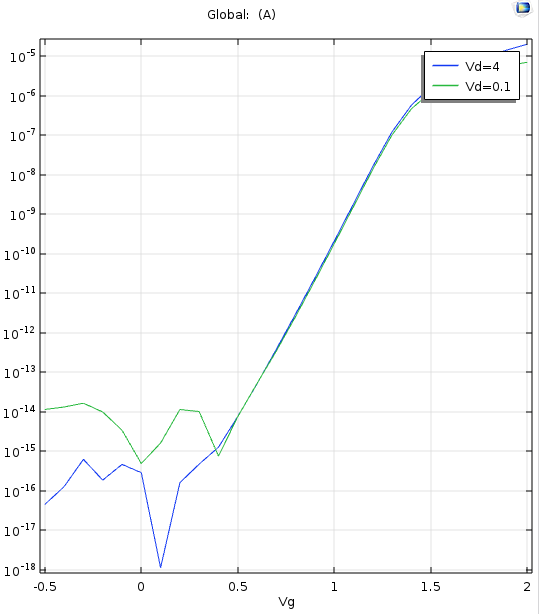
\includegraphics[width=0.7\textwidth]{mosfet_lab1_1_6um_id_vs_vg.png}}
  \caption{Id vs Vg for 1.6um.}
  \label{fig:idvg130_1}
\end{figure}
\begin{figure}[!ht]
  \centering
  \noindent\makebox[\textwidth]{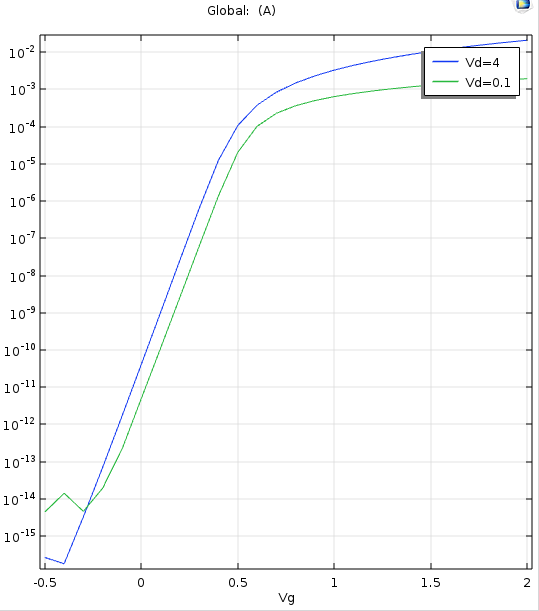
\includegraphics[width=0.7\textwidth]{mosfet_lab1_130nm_id_vs_vg.png}}
  \caption{Id vs Vg for 130nm.}
  \label{fig:idvg130_1}
\end{figure}

\section{Task 2}
The DIBL effect can be reduced by reducing the substrate doping.
In the COMSOL design this means that we should decrease the doping concentration for \textit{Analytic Doping Model 1}.
However, the simulation fails if the doping concentrations are changed and I can not figure out why so I can not show it.
The course book talks about DIBL on pages 333 --- 335, where it also states that the doping concentration should be reduced to widen the depletion width, thereby partially mitigating the short-channel effect.
\end{document}